\section{ETL}\label{sec:ETL}
The data foundation for this project relies on two sources, refer section \ref{sec:datafound}. Extract-Transform-Load (ETL) is an important phase for integrating these two sources of information into the data warehouse while ensuring a uniform data-representation. A preprocessing procedure fills static support-tables and dimensions with data. The data available through OpenStreetMap and the INFATI project contains necessities for car information and enough information to start building a GPS Fact. After the preliminary data is loaded into the data warehouse, a number of post-processing procedures fills the remaining tables with data. An overview of the ETL-procedure can be seen in Figure \ref{fig:etl}.

\begin{figure}[tb]
\centering
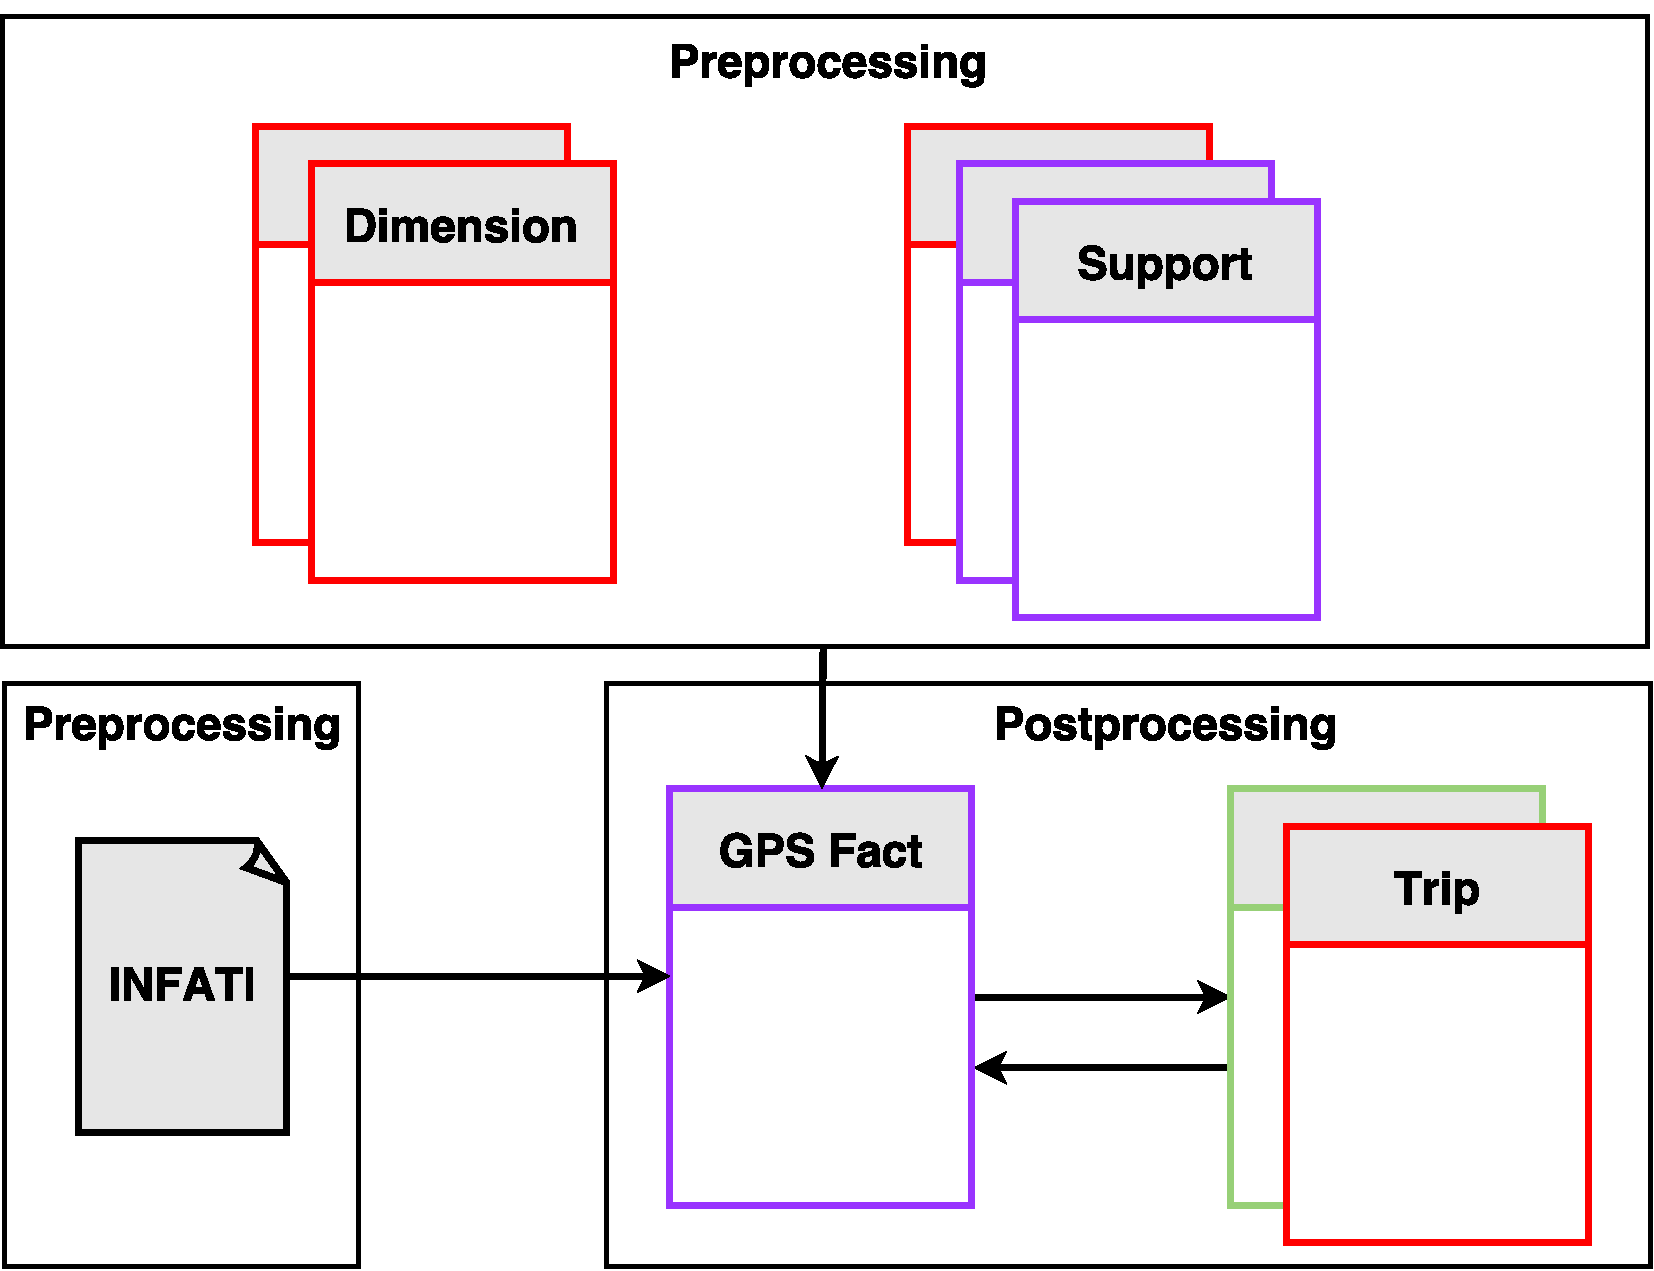
\includegraphics[width=0.465\textwidth]{Pictures/ETL}
\caption{Dataflow throughout the ETL process}
\label{fig:etl}
\end{figure}

The INFATI project\cite{art:INFATI} uses a digital roadmap from OpenStreetMap\cite{osm}. The same digital roadmap is used for this project. A few modifications is introduced, like storing the column \textit{direction} as a smallint instead of a textual representation. 

The INFATI dataset\cite{art:INFATI} contains 17 columns of data, separated by a varying number of spaces. Due to the natural challenges of map-matching, some entries have not been map-matched successfully. These rows contain only 14 columns of data. This renders the dataset unreadable, due to problems with trailing zeros, when loading with a space-separator. To ease the ETL process, a script was made to change and fix the separator. In this script \# is used as delimiter, and whenever a row was not map-matched, three \#'s are appended to that row.

INFATI coordinate-sets are stored in the geodetic datum ED50, within UTM zone 32N. The system proposed in this paper is built on GPS, and a transformation from UTM to lattitude and longitude is needed. Coordinate-sets are stored as points, lines or polygons and stored in the data warehouse as PostGIS\cite{postgis} geometries. These geometries has to be assigned the correct spatial reference system identifier(SRID), in order to display a position correctly. With the INFATI dataset being logged in ED50 and UTM zone 32N, this corresponds to a SRID of 23032\cite{UTM32N}. Latitude and longitude format is part of World Geodetic System(WGS), latest edition being WGS84 and has SRID 4326\cite{WGS84}. To transform the INFATI data into the desired format the geometry is created, assigned the appropriate SRID of 23032, and then transformed into latitude and longitude format using the SRID of 4326. 

Appropriate data for the support table \textit{Quality Information} and the dimensions \textit{Date} and \textit{Time} are computed and stored. For \textit{Quality Information} this means storing combinations of HDOP and satellites.

The preprocessing is now complete, and the INFATI data can be loaded into the data warehouse. A car must be created and stored in \textit{Car Information} table. Hereafter the corresponding INFATI data is loaded into the \textit{GPS Fact} table. 

Three postprocessing-steps will now fill in measures which will make it possible to determine the cost of a trip. 

The first step is dividing the batch of gpsfacts into trips for each car. Each found trip will be stored in an empty Trip Fact. The empty trip will then be assigned the appropriate CarId for the trip, an auto-incremented TripId, and the gpsfacts belonging to that calculated trip will be updated with the assigned TripId. The process of dividing gpsfacts into trips is done by fetching them from the data warehouse, and sort them based on their timestamp. A new instance of a trip class is created, and gpsfacts are continuously stored into this instance. When a timestamp is encountered, that is more than three minutes older than the previous, a new instance of the trip class is instantiated. This process is repeated until all gpsfacts belong to a trip. These trips are then used to store tripfacts and update gpsfacts.

The second step is calculating measures for gpsfacts. The process runs through a triple nested loop by walking through all gpsfacts of all trips of all cars. Measures are then calculated for every single gpsfact within the context of a trip. In practise a query is made to retrieve all gpsfacts belonging to a trip in ascending order according to timestamps. A loop will then repeat from the second entry towards the end of the trip, calculating measures based on what has happened since the previous entry. It is metrics like acceleration change, and meters driven that will be stored in this process. At the end of the process these gpsfacts will be updated in the data warehouse.

The third step begins when the \textit{GPS Fact} is updated with measures, because this makes it possible to compute measures for entries in the Trip Fact table. This process is another triple nested loop walking through the gpsfacts of every trip of every car. Combining the information found in gpsfacts, summarized measures can be updated in the tripfact. Then intervals defined in tripfacts are populated with appropriate percentages, relative to the total counts, based on the distribution of severity of delinquencies. Additionally, basic measures like when the trip started, total meters driven, etc. are calculated. When all the measures are calculated, the trip is updated in the data warehouse.

\textit{SubTrip Fact} is only conceptual at this time. Nothing is calculated or stored in the data warehouse. Given the similarities between \textit{SubTrip Fact} and \textit{SubTrip Fact}, it would however use many of the same computations as \textit{TripFact} which would make this process relatively trivial.

If a data source other than INFATI were to be used in the future, some of the ETL procedure would have to be redesigned, as some of the implementation is written specifically to handle the INFATI data. As such we would need another process for transforming the data into the uniform data-representation present in the data warehouse.

%Måske skal det her ikke med?
To decrease the computation time of the ETL phase, the loading process runs on multiple threads so that a single car is being loaded in its own thread. This is only relevant for the INFATI dataset. In a working setting, data would come in bulks of single trips. 